\documentclass{article}

\usepackage{graphicx}
\usepackage{tikz}
\usepackage{tikzsymbols}
\usetikzlibrary{calc,patterns,shapes.geometric}
\pagestyle{empty}
\usepackage[margin=0pt]{geometry}
\geometry{papersize={14in,12in}}

\def\centerarc[#1](#2)(#3:#4:#5){\draw[#1] ($(#2)+({#5*cos(#3)},{#5*sin(#3)})$) arc (#3:#4:#5);}

\begin{document}
	\begin{figure}
		\centering
		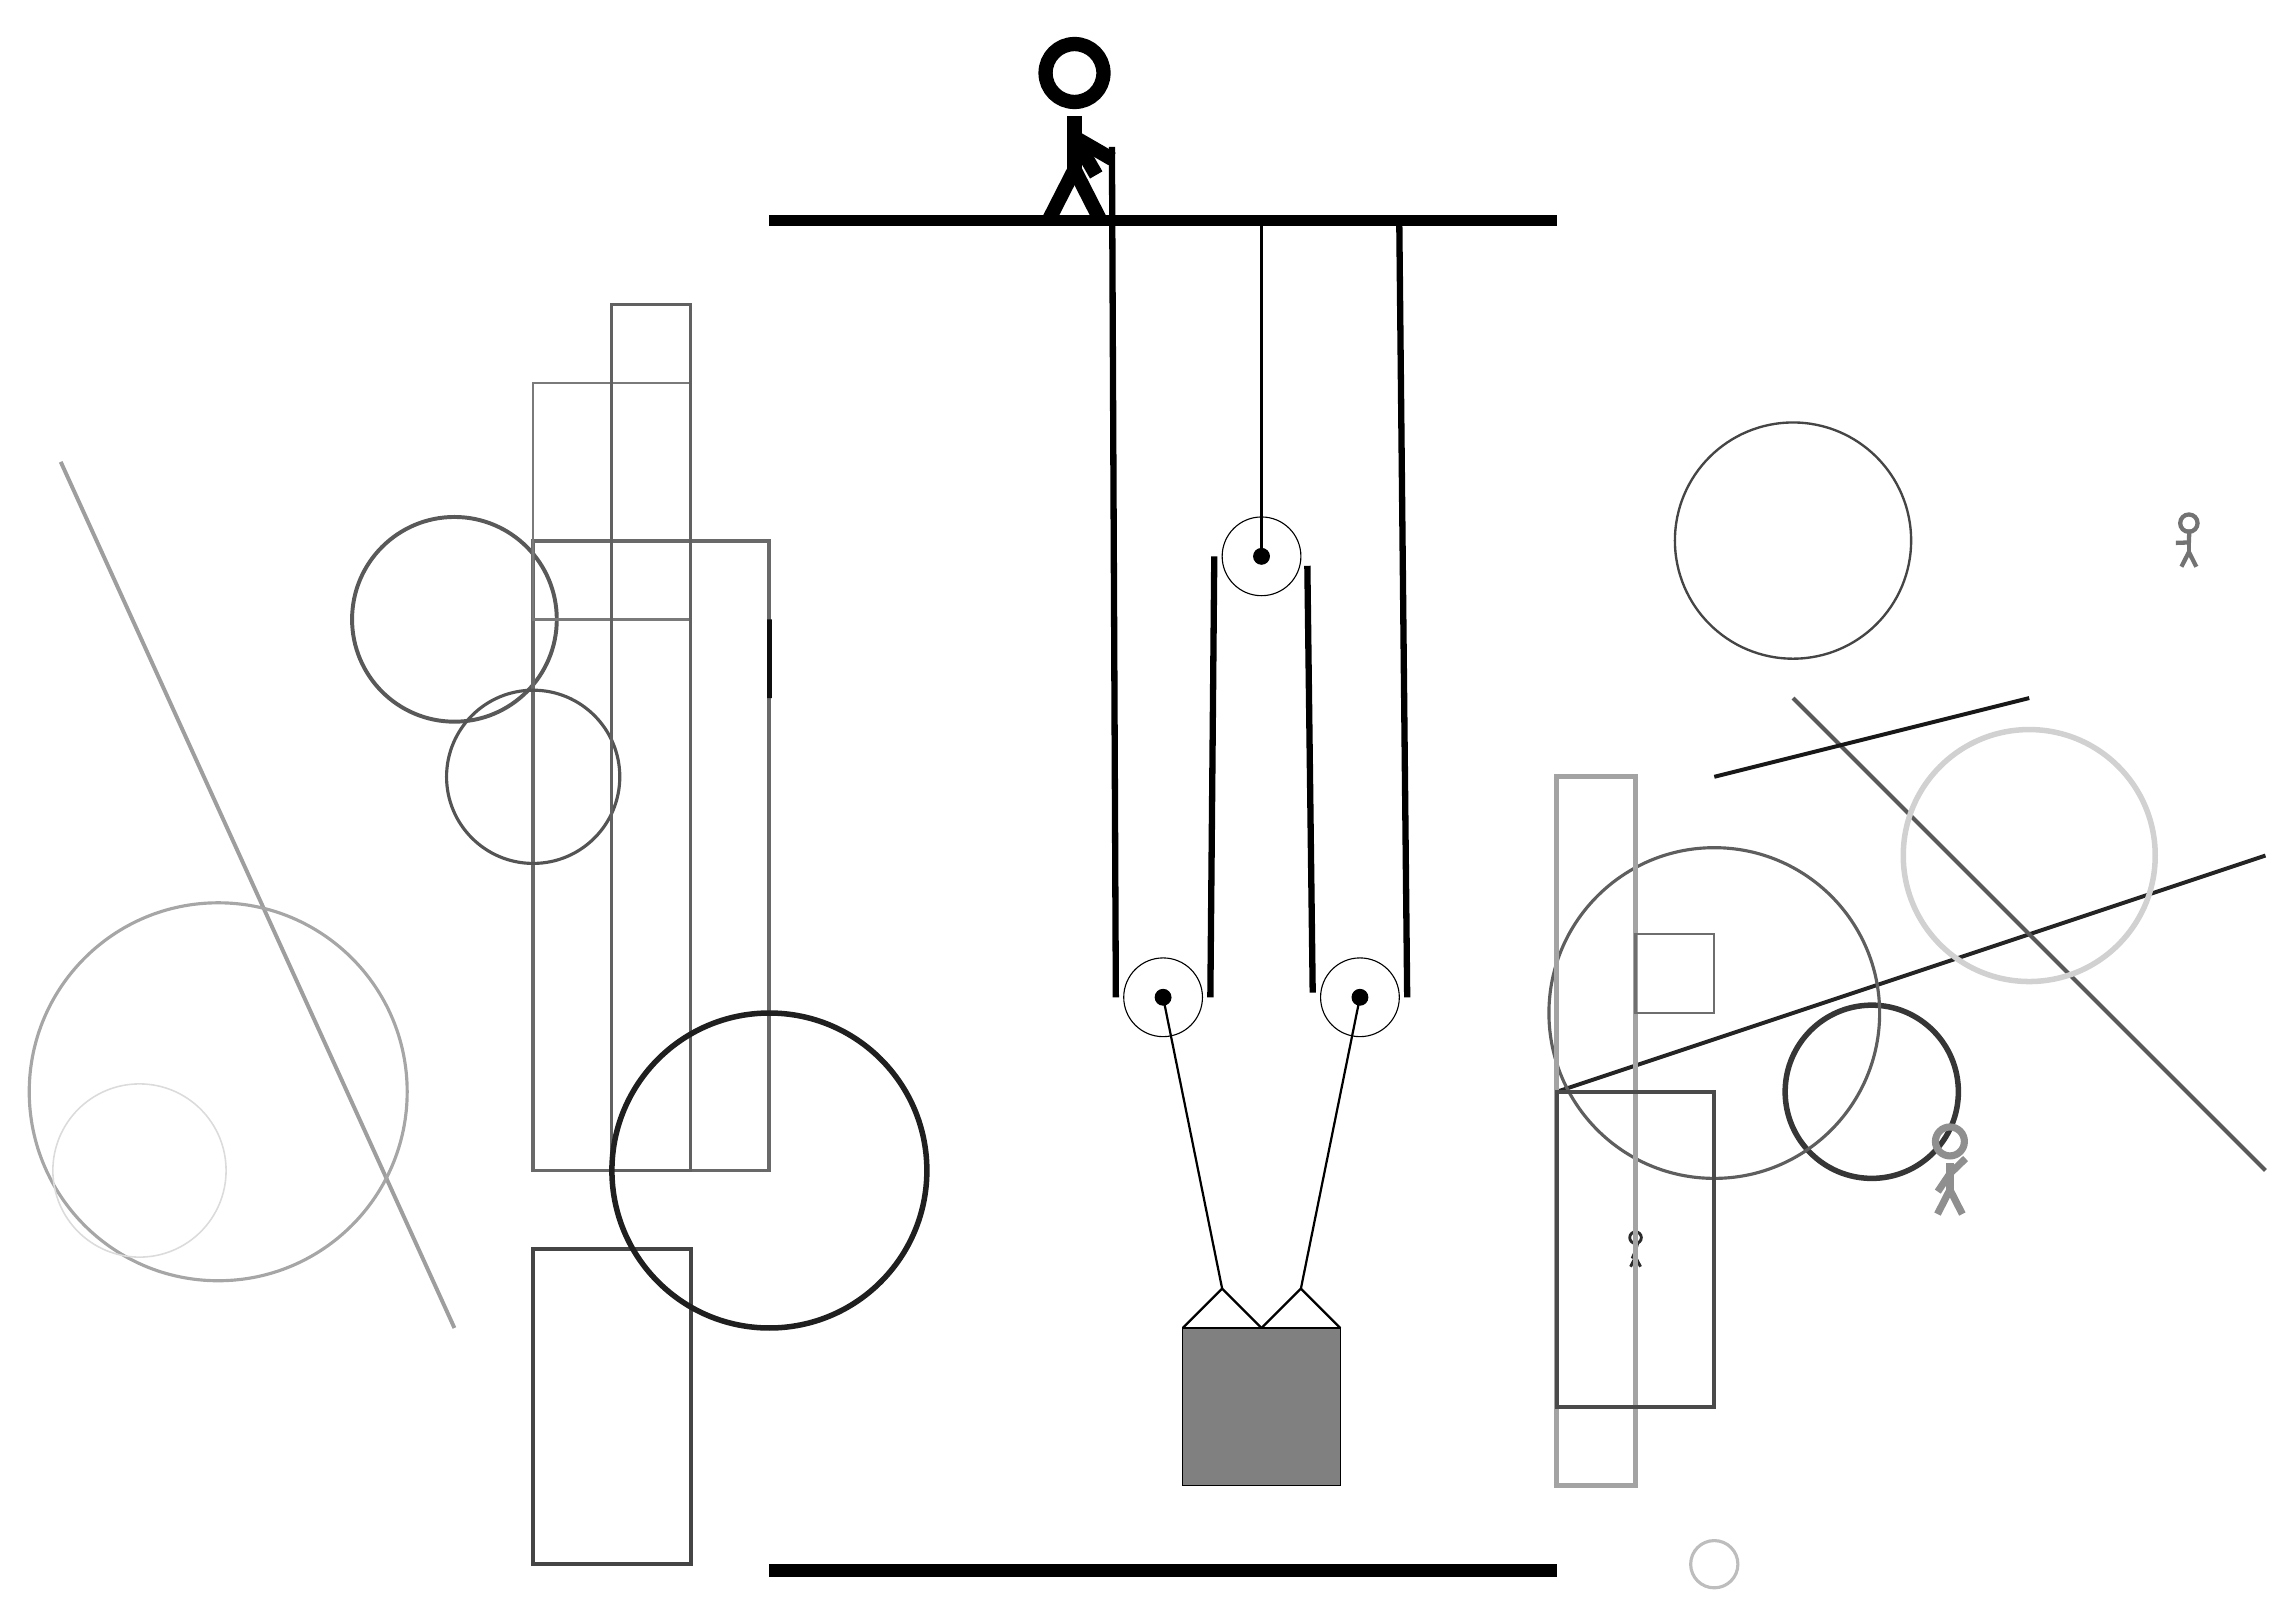
\begin{tikzpicture}
			%%%%% START %%%%%
			
			\draw[fill=black] (-4, 14) rectangle (6, 14.125);
			
			\draw (1, 4.2) circle (0.5);
			\draw[fill=black] (1, 4.2) circle (0.1);
			
			\draw (2.25, 9.8) circle (0.5);
			\draw[fill=black] (2.25, 9.8) circle (0.1);
			\draw[thick] (2.25, 9.8) -- (2.25, 14);
			
			\draw (3.5, 4.2) circle (0.5);
			\draw[fill=black] (3.5, 4.2) circle (0.1);
			
			\draw[thick] (3.5, 4.2) -- (2.75, 0.5);
			\draw[thick] (1, 4.2) -- (1.75, 0.5);
			\draw[thick]  (1.25, 0) -- (1.75, 0.5) -- (2.25, 0);
			\draw[thick]  (2.25, 0) -- (2.75, 0.5) -- (3.25, 0);
			\draw[fill=black!50] (1.25, 0) rectangle (3.25, -2);
			
			\draw[line width=0.8mm] (0.35, 15) --  (0.4, 4.2);
			\centerarc[line width=0.8mm](1, 4.2)(180:360:0.6);
			\draw[line width=0.8mm] (1.6, 4.2) -- (1.65, 9.8);
			\centerarc[line width=0.8mm](2.25, 9.8)(-20:180:0.6);
			\draw[line width=0.8mm](2.832, 9.68) -- (2.9, 4.26);
			\centerarc[line width=0.8mm](3.5, 4.2)(160:360:0.6);
			\draw[line width=0.8mm](4.1, 4.2) -- (4.0, 14);
			
			\draw [line width=0.4mm, color=black!99](-4, 0) circle (0.0);
			
			\draw [line width=0.3mm, color=black!73](9, 10) circle (1.5);
			\draw[line width=0.5mm, color=black!86](6, 3) -- (15, 6);
			\draw [line width=0.5mm, color=black!65](-8, 9) circle (1.3);
			
			\draw [line width=0.7mm, color=black!79](10, 3) circle (1.1);
			\draw [line width=0.4mm, color=black!63](8, 4) circle (2.1);
			
			\node[line width=0.5mm, color=black!44] at (11, 2) {\Strichmaxerl[5][56][44]};
			\draw[line width=0.5mm, color=black!59] (-4, 2) rectangle (-7, 10);
			\draw [line width=0.4mm, color=black!67](-7, 7) circle (1.1);
			\node[line width=0.2mm, color=black!83] at (7, 1) {\Strichmaxerl[2][67][73]};
			\draw[line width=0.5mm, color=black!65](9, 8) -- (15, 2);
			
			\draw [line width=0.4mm, color=black!26](8, -3) circle (0.3);
			\node[line width=0.6mm, color=black!55] at (14, 10) {\Strichmaxerl[3][2][88]};
			
			\draw[line width=0.5mm, color=black!38](-8, 0) -- (-13, 11);
			\draw[line width=0.5mm, color=black!91](8, 7) -- (12, 8);
			\draw [line width=0.7mm, color=black!18](12, 6) circle (1.6);
			
			\draw[line width=0.3mm, color=black!52] (-5, 9) rectangle (-7, 12);
			\draw[line width=0.5mm, color=black!73] (-5, 1) rectangle (-7, -3);
			\draw[line width=0.6mm, color=black!36] (6, -2) rectangle (7, 7);
			\draw[line width=0.4mm, color=black!62] (-5, 2) rectangle (-6, 13);
			\draw [line width=0.4mm, color=black!35](-11, 3) circle (2.4);
			
			\draw[line width=0.5mm, color=black!71] (6, 3) rectangle (8, -1);
			\draw[line width=0.7mm, color=black!94] (-4, 8) rectangle (-4, 9);
			\draw[line width=0.3mm, color=black!57] (7, 4) rectangle (8, 5);
			\draw [line width=0.7mm, color=black!88](-4, 2) circle (2.0);
			
			\draw [line width=0.5mm, color=black!41](11, 7) circle (0.0);
			\draw [line width=0.2mm, color=black!14](-12, 2) circle (1.1);
			
			\node at (-0.07, 15.2) {\Strichmaxerl[10][120][-30]};
			
			\draw[fill=black] (-4, -3) rectangle (6, -3.15);
			
			%%%%% END %%%%%
		\end{tikzpicture}
	\end{figure}	
\end{document}